\documentclass [11pt, a4paper, oneside] {article}
\usepackage {amsmath}
\usepackage {geometry}
\geometry{left=2.5cm,right=2.5cm}
\usepackage {amssymb}
\usepackage {graphicx}
\usepackage{multirow}
\linespread{1.5}
\usepackage[procnames]{listings}
\usepackage{color}
\author {Yue Wang, A53102167}
\title {CSE250A Homework2 Answer}
\begin {document}
\maketitle
\section *{2.1 Probabilistic Inference}
\subsection *{(a)}
$P(A=1, E=1, B=0)  = P(A=1|E=1, B=0)*P(E=1)*P(B=0) = P(A=1|E=1, B=0)*P(E=1)*(1-P(B=1)) = 0.29*0.002*(1-0.001) = 0.00057942$\\
$P(A=1, E=1, B=1) =  P(A=1|E=1, B=1)*P(E=1)*P(B=1) = 0.95*0.002*0.001 = 0.0000019$\\
$P(A=1, E=1) = P(A=1, E=1, B=0) + P(A=1, E=1, B=1) = 0.00057942 + 0.0000019 = 0.00058132$\\
$P(A=1, E=0, B=0) = P(A=1|E=0, B=0)*P(E=0)*P(B=0) = P(A=1|E=0, B=0)*(1-P(E=1))*(1-P(B=1)) = 0.001*(1-0.002)*(1-0.001) = 0.000997$\\
$P(A=1, E=0, B=1) = P(A=1|E=0, B=1)*P(E=0)*P(B=1) = P(A=1|E=0, B=1)*(1-P(E=1))*P(B=1) = 0.94*(1-0.002)*0.001 = 0.000938$\\
$P(A=1, E=0) = P(A=1, E=0, B=0) + P(A=1, E=0, B=1) = 0.000997 + 0.000938 = 0.001935$\\
$P(A=1) = P(A=1, E=1) + P(A=1, E=0) = 0.00058132 + 0.001935 = 0.00252$\\
$P(E=1|A=1) = \frac{P(A=1, E=1)}{P(A=1)} = \frac{0.00058132}{0.00252} = 0.231$\\
\subsection *{(b)}
$P(A=1|B=1) = \frac{P(A=1, B = 1)}{P(B=1)} = \frac{P(A=1, E=1, B=1) + P(A=1, E=0, B=1)}{P(B=1)} = \frac{0.0000019+0.000938}{0.001} = 0.9399$\\
$P(E=1|A=1, B=1) = \frac{P(A=1|E=1, B=1)*P(E=1|B=1)}{P(A=1|B=1)} = \frac{P(A=1|E=1, B=1)*P(E=1)}{P(A=1|B=1)} = \frac{0.95*0.002}{0.9399} = 0.00202$\\
\subsection *{(c)}
$P(A=0) = 1 - P(A=1) = 1 - 0.00252 = 0.99748$\\
$P(J=1) = P(J=1, A=0) + P(J=1, A=1) = P(J=1|A=0)*P(A=0) + P(J=1|A=1)*P(A=1) = 0.05*0.99748 + 0.90*0.00252 = 0.052142$\\
$P(J=0) = 1 - P(J=1) = 1 - 0.052142 = 0.947858$\\
$P(A=1|J=0) = \frac{P(J=0| A=1)*P(A=1)}{P(J=0)} = \frac{(1-P(J=1|A=1))*P(A=1)}{P(J=0)} = \frac{(1-0.90)*0.00252}{0.947858} = 0.0002659$\\
\subsection *{(d)}
$P(M=0|A=0) = 1 - P(M=1|A=0) = 0.99$\\
$P(M=0|A=1) = 1 - P(M=1|A=1) = 0.70$\\
$P(M=0) = P(M=0, A=1) + P(M=0, A=1) = P(M=0|A=0)*P(A=0) + P(M=0|A=1)*P(A=1) = 0.99*0.99748 + 0.70*0.00252 = 0.9892692$\\
$P(A=1|M=0) = \frac{P(M=0|A=1)*P(A=1)}{P(M=0)} = \frac{0.70*0.00252}{0.9892692} = 0.001783134$\\
$P(A=0|M=0) = 1 - P(A=1|M=0) = 0.998216866$\\
$P(J=0|M=0) = P(J=0, A=1|M=0) + P(J=0, A=0|M=0) = P(J=0|A=1, M=0)*P(A=1|M=0) + P(J=0|A=0, M=0)*P(A=0|M=0) = P(J=0|A=1)*P(A=1|M=0) + P(J=0|A=0)*P(A=0|M=0)=
(1-0.90)*0.001783134 + (1-0.05)*0.998216866 = 0.948484336$\\
$P(A=1|J=0, M=0) = \frac{P(J=0|A=1, M=0)*P(A=1|M=0)}{P(J=0|M=0)} = \frac{P(J=0|A=1)*P(A=1|M=0)}{P(J=0|M=0)} = \frac{(1-0.90)*0.001783134}{0.948484336} = 0.000188$\\
\subsection *{(e)}
$P(A=1|M=1) = \frac{P(M=1|A=1)*P(A=1)}{P(M=1)} = \frac{P(M=1|A=1)*P(A=1)}{1 - P(M=0)} = \frac{0.70*0.00252}{1-0.9892692} = 0.164387$\\
\subsection *{(f)}
$P(A=1|E=0) = \frac{P(E=0|A=1)*P(A=1)}{P(E=0)} = \frac{(1-0.231)*0.00252}{(1-0.002)} = 0.001941764$\\
$P(A=0|E=0) = 1 - P(A=1|E=0) = 1 - 0.001941764 = 0.998058236$\\
$P(M=1|E=0) = P(M=1, A=1|E=0) + P(M=1, A=0|E=0) = P(M=1|A=1, E=0)*P(A=1|E=0) + P(M=1|A=0, E=0)*P(A=0|E=0) = P(M=1|A=1)*P(A=1|E=0) + P(M=1|A=0)*P(A=0|E=0) = 
0.70*0.001941764 + 0.01*0.998058236 = 0.011339817$\\
$P(A=1|M=1, E=0) = \frac{P(M=1|A=1, E=0)*P(A=1|E=0)}{P(M=1|E=0)} = \frac{P(M=1|A=1)*P(A=1|E=0)}{P(M=1|E=0)} = \frac{0.70*0.001941764}{0.011339817} = 0.119864$\\

The result is consistent with the commonsense. From (a) and (b), we know burglary explain away the alarm, which decrease the probability of earthquake. From (c) and (d),  the probability of earthquaking occurring is smaller when John and Mary don't call than that when one of John and Mary calls. From (e) and (f), when we know the earthquake didn't happen, we have less confidence in alarm going off. 
\section *{2.2 Probabilistic reasoning}
\subsection *{(a)}
$r_k = \frac{P(D=0|S_1=1, S_2=1, \cdots, S_k=1)}{P(D=1|S_1=1, S_2=1, \cdots, S_k=1)} = \frac{\frac{P(S_1=1, S_2=1, \cdots, S_k=1|D=0)*P(D=0)}{P(S_1=1, S_2=1, \cdots, S_k=1)}}{\frac{P(S_1=1, S_2=1, \cdots, S_k=1|D=1)*P(D=1)}{P(S_1=1, S_2=1, \cdots, S_k=1)}} = \frac{P(S_1=1, S_2=1, \cdots, S_k=1|D=0)*P(D=0)}{P(S_1=1, S_2=1, \cdots, S_k=1|D=1)*P(D=1)} =\frac{P(S_1=1, S_2=1, \cdots, S_k=1|D=0)}{P(S_1=1, S_2=1, \cdots, S_k=1|D=1)} =  \frac{P(S_1|D=0)*P(S_2|D=0)*\cdots*P(S_k|D=0)}{P(S_1|D=1)*P(S_2|D=1)*\cdots*P(S_k|D=1)} = \frac{1*\frac{1}{5}*\frac{5}{7}*\cdots*\frac{2^{k-1}+(-1)^{k-1}}{2^k+(-1)^k}}{\frac{1}{2}*\frac{1}{2}*\cdots*\frac{1}{2}} = \frac{\frac{1}{2^k+(-1)^k}}{(\frac{1}{2})^k} = \frac{1}{1+(-\frac{1}{2})^k}$\\
The result shows that the doctor's diagnosis depend on whether the day is odd number or even number. If it is odd number, the doctor diagnoses the patient with the D=0, otherwise with D=1.
\subsection *{(b)}
The result depends on whether the day is even number or odd number. But with more symptoms observed, the diagnosis is less certain. Because with more symptoms observed, the denominator of $r_k$ is getting closer to 1, which leads to the $r_k$ getting closer to 1. So the result is less certain.\\ 
\section *{2.3 Sigmoid function}
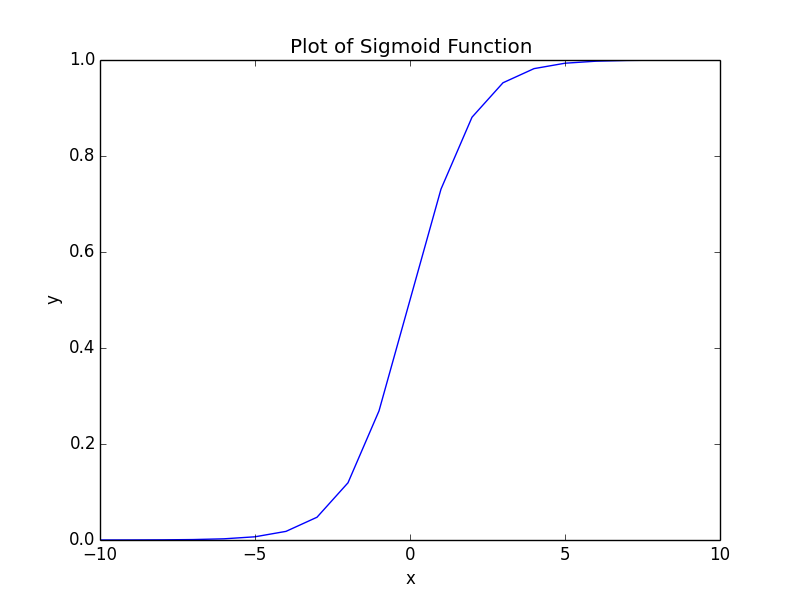
\includegraphics[height=5cm]{figure_1.png}
\subsection *{(a)}
$\sigma'(z) = e^z*(\frac{1}{1+e^{-z}})^2 = \frac{1}{1+e^{-z}}*\frac{e^{-z}}{1+e^{-z}} =  \frac{1}{1+e^{-z}}*\frac{e^{-z}*e^{z}}{(1+e^{-z})*e^{z}} = \frac{1}{1+e^{-z}}*\frac{1}{1+e^{z}} = \sigma(z)\sigma(-z)$\\
\subsection *{(b)}
$\sigma(-z) + \sigma(z) = \frac{1}{1+e^{-z}} + \frac{1}{1+e^{z}} = \frac{e^z}{e^z+1} + \frac{1}{1+e^{z}} = \frac{1+e^{z}}{1+e^{z}} = 1$\\
\subsection *{(c)}
$L(\sigma(z)) = \log(\frac{\sigma(z)}{1-\sigma(z)}) = \log(\frac{\sigma(z)}{\sigma(-z)}) = \log(\frac{1+e^z}{1+e^{-z}}) = \log(\frac{(1+e^z)*e^{-z}}{(1+e^{-z})*e^{-z}}) = \log(\frac{(1+e^{-z})}{(1+e^{-z})*e^{-z}}) = \log(\frac{1}{e^{-z}})= \log(e^z) = z$
\section *{2.4 Conditional independence}
1.$P(rain, sprinkler|month) = P(rain|month)P(sprinkler|month)$\\
2.$P(month, water|sprinkler) = P(month|sprinkler)P(water|sprinkler)$\\
3.$P(month, water|rain) = P(month|rain)P(water|rain)$\\
4.$P(month, water|sprinkler, rain) = P(month|sprinkler, rain)P(water|sprinkler, rain)$\\
5.$P(sprinkler, fall|water) = P(sprinkler|water)P(fall|water)$\\
6.$P(rain, fall|water) = P(rain|water)P(fall|water)$\\
7.$P(month, fall|sprinkler, water) = P(month|sprinkler, water)P(fall|sprinkler, water)$\\
8.$P(month, fall|rain, water) = P(month|rain, water)P(fall|rain, water)$\\
9.$P(month, fall|sprinkler, rain) = P(month|sprinkler, rain)P(fall|sprinkler, rain)$\\
10.$P(month, fall|sprinkler, rain, water) = P(month|sprinkler, rain, water)P(fall|sprinkler, rain, water)$\\
11.$P(month, fall|sprinkler) = P(month|sprinkler)P(fall|sprinkler)$\\
12.$P(month, fall|rain) = P(month|rain)P(fall|rain)$\\
13.$P(month, fall|water) = P(month|water)P(fall|water)$\\
14.$P(month, water|sprinkler, fall) = P(month|sprinkler, fall)P(water|sprinkler, fall)$\\
15.$P(month, water|rain, fall) = P(month|rain, fall)P(water|rain, fall)$\\
16.$P(month, water|sprinkler, rain, fall) = P(month|sprinkler, rain)P(water|sprinkler, rain, fall)$\\
\section *{2.5 Markov blanket}
There are 5 types conditional independence, let's look at each case:\\
Parent's parents $->$ X:\\
$P(1, X|B_X) = P(1|B_X)P(X|B_X)$ for the d-separation rule (II)\\
Children's parent's parents $->$ X:\\
$P(2, X|B_X) = P(2|B_X)P(X|B_X)$ for the d-separation rule (II), this seems strange because in the path $2->X$, the rule (III) doesn't hold. But in the definition of d-separation, one of the three rules holds will lead to d-separation. (Since 2 and X are not d-connected because there is a "non-collider" in the path)\\
Parent's children $->$ X:\\
$P(3, X|B_X) = P(3|B_X)P(X|B_X)$ for the d-separation rule (I)\\
Children's parent's children $->$ X:\\
$P(4, X|B_X) = P(4|B_X)P(X|B_X)$ for the d-separation rule (II) and similar explaination with 2$->$X\\
Children's children $->$ X:\\
$P(5, X|B_X) = P(5|B_X)P(X|B_X)$ for the d-separation rule (II)\\
\section *{2.6 Noisy-OR}
(a)$P(Z=1|X=0, Y=0) < P(Z=1|X=0, Y=1)$\\
(b)$P(Z=1|X=1, Y=0) < P(Z=1|X=0, Y=1)$\\
(c)$P(Z=1|X=1, Y=0) < P(Z=1|X=1, Y=1)$\\
(d)$P(X=1) < P(X=1|Z=1)$\\
(e)$P(X=1) = P(X=1|Y=1)$\\
(f)$P(X=1|Z=1) > P(X=1|Y=1, Z=1)$\\
(g)$P(X=1)P(Y=1)P(Z=1) < P(X=1, Y=1, Z=1)$\\
\section *{2.7 More conditional independence}
True\qquad P(E, F|D) = P(E|D)P(F|D) \\
False\qquad P(E, F|C, D) = P(E|C, D)P(F|C, D)\\
True \qquad P(E, F|A, B, D) = P(E|A, B, D)P(F|A, B, D)\\
False \qquad P(D|C) = P(D)\\
True \qquad P(D|A,B) = P(D|A, B, C)\\
True \qquad P(A, B) = P(A)P(B)\\
False \qquad P(A|C, D) = P (A|C, D, F)\\
True \qquad P(A|B, C, D) = P(A|B, C, D, F)\\
True \qquad P(B|A, C, D, F) = P(B|A, C, D, F, E)\\
False \qquad P(B, F, A, E|C, D) = P(B, F|C, D)P(A, E|C, D)\\
\section *{2.8 Even more conditional independence}
$P(B|D) = P(B|S) \qquad S = {D, G, A, C, E}$\\
$P(B|D, F) = P(B|S) \qquad S = {D, F, G, E}$\\
$P(C|D) = P(C|S) \qquad S = {D, B, G}$\\
$P(C|F, G) = P(C|S) \qquad S = {F, G}$\\
$P(C|A, E, F) = P(C|S) \qquad S = {A, E, F}$\\
$P(E|F) = P(E|S) \qquad S = {F}$\\
$P(E|C) = P(E|S) \qquad S = {C, A, F, B, D, G}$\\
$P(F) = P(F|S) \qquad S = {}$\\
$P(F|C, D) = P(F|S) \qquad S = {C, D, E, G}$\\
$P(A, B) = P(A, B|S) \qquad S = {}$\\
\end{document}